% Guía de usuario de MICD (visor web) — para personal médico.
% Compilar con:  latexmk -pdf guia-usuario.tex   (las capturas están en img/)
\documentclass[11pt,a4paper]{report}

\usepackage[utf8]{inputenc}
\usepackage[T1]{fontenc}
\usepackage[spanish,es-noshorthands,es-nolists]{babel}

% ── Tipografía: Inter (la de la aplicación) + Source Code Pro ──────────────
\usepackage[type1]{inter}
\renewcommand{\familydefault}{\sfdefault}
\usepackage[scale=0.88]{sourcecodepro}
\usepackage[final,tracking=false,kerning=true,spacing=true]{microtype}
\linespread{1.12}

\usepackage[a4paper,top=2.9cm,bottom=2.6cm,left=2.6cm,right=2.6cm,
  headheight=16pt,headsep=0.9cm,footskip=1.2cm]{geometry}
\usepackage{graphicx}
\usepackage[table]{xcolor}
\usepackage[most]{tcolorbox}
\usepackage{tikz}
\usetikzlibrary{calc,positioning,babel}
\usepackage{enumitem}
\usepackage{titlesec}
\usepackage{titletoc}
\usepackage{fancyhdr}
\usepackage{booktabs}
\usepackage{tabularx}
\usepackage{longtable}
\usepackage{float}
\usepackage{fontawesome5}
\usepackage[font={small},labelfont={bf},labelsep=period,skip=8pt]{caption}
\usepackage{hyperref}

\graphicspath{{img/}}

% ── Paleta (derivada de la aplicación) ─────────────────────────────────────
\definecolor{micd}{HTML}{1FA67A}      % esmeralda, legible sobre papel
\definecolor{micdbright}{HTML}{2EE6A8}% acento de la app (sobre fondo oscuro)
\definecolor{micddeep}{HTML}{0F6E52}  % esmeralda oscuro para texto
\definecolor{micddark}{HTML}{0D0F11}  % fondo de la app
\definecolor{micdpanel}{HTML}{16191D}
\definecolor{ink}{HTML}{1C2228}
\definecolor{muted}{HTML}{66707A}
\definecolor{hair}{HTML}{DDE3E8}
\definecolor{soft}{HTML}{F4F7F8}
\definecolor{warn}{HTML}{C0392B}
\definecolor{tipbg}{HTML}{EDF9F4}
\definecolor{warnbg}{HTML}{FDF0EF}

\color{ink}
\hypersetup{colorlinks=true,linktoc=page,linkcolor=micddeep,urlcolor=micddeep,
  pdftitle={MICD — Guía de usuario},pdfauthor={UBA — FIUBA}}

\setlength{\parindent}{0pt}
\setlength{\parskip}{0.55em plus 0.15em}
\arrayrulecolor{hair}
\setlength{\aboverulesep}{0.5ex}
\setlength{\belowrulesep}{0.6ex}
\renewcommand{\arraystretch}{1.25}
\captionsetup{labelfont={bf,color=micddeep},textfont={color=muted}}

% ── Títulos ────────────────────────────────────────────────────────────────
\newcommand{\chaptitle}[1]{%
  \begin{minipage}[b]{0.78\linewidth}
    {\color{micd}\small\bfseries\MakeUppercase{\chaptertitlename}\par}
    \vspace{3pt}
    {\raggedright\hyphenpenalty=10000\exhyphenpenalty=10000\fontsize{26}{31}\selectfont\bfseries\color{ink}#1\par}
  \end{minipage}}
\titleformat{\chapter}[block]
  {\normalfont}
  {\begin{tikzpicture}[baseline=(n.south)]
     \node[fill=micd,rounded corners=7pt,minimum width=1.6cm,minimum height=1.6cm,
           text=white,font=\fontsize{30}{30}\selectfont\bfseries] (n) {\thechapter};
   \end{tikzpicture}}
  {16pt}
  {\chaptitle}
  [\vspace{10pt}{\color{hair}\titlerule[1pt]}]
\titleformat{name=\chapter,numberless}[block]
  {\normalfont\fontsize{26}{30}\selectfont\bfseries\color{ink}}{}{0pt}{}
  [\vspace{6pt}{\color{hair}\titlerule[1pt]}]
\titlespacing*{\chapter}{0pt}{0pt}{28pt}

\titleformat{\section}
  {\normalfont\Large\bfseries\color{ink}\raggedright}
  {\textcolor{micd}{\thesection}}{0.8em}{}
  [\vspace{-7pt}{\color{micd}\rule{2.2em}{2pt}}]
\titleformat{name=\section,numberless}
  {\normalfont\Large\bfseries\color{ink}}{}{0pt}{}
  [\vspace{-7pt}{\color{micd}\rule{2.2em}{2pt}}]
\titlespacing*{\section}{0pt}{20pt}{8pt}

\titleformat{\subsection}
  {\normalfont\large\bfseries\color{micddeep}}
  {\thesubsection}{0.7em}{}
\titleformat{name=\subsection,numberless}
  {\normalfont\large\bfseries\color{micddeep}}
  {\textcolor{micd}{\rule[0.15ex]{4pt}{0.9em}}}{0.5em}{}
\titlespacing*{\subsection}{0pt}{14pt}{4pt}

% ── Índice ─────────────────────────────────────────────────────────────────
\titlecontents{chapter}[2.6em]
  {\addvspace{7pt}\bfseries\color{ink}}
  {\contentslabel[\textcolor{white}{\colorbox{micd}{\makebox[1.1em]{\small\thecontentslabel}}}]{2.6em}}
  {}
  {\hfill\textcolor{micd}{\contentspage}}
\titlecontents{section}[5.4em]
  {\addvspace{1pt}\color{ink}}
  {\contentslabel[\textcolor{muted}{\thecontentslabel}]{2.8em}}
  {}
  {\textcolor{hair}{\titlerule*[0.6em]{.}}\textcolor{muted}{\contentspage}}

% ── Encabezado y pie ───────────────────────────────────────────────────────
\newcommand{\pagepill}{%
  \tikz[baseline=(p.base)]\node[fill=soft,draw=hair,rounded corners=7pt,
    inner xsep=8pt,inner ysep=3pt,font=\footnotesize\bfseries,text=micddeep] (p) {\thepage};}
\pagestyle{fancy}
\fancyhf{}
\fancyhead[L]{\footnotesize\bfseries\textcolor{micd}{\faCircle[regular]}\ \ \textcolor{ink}{MICD}\textcolor{muted}{\ \ ·\ \ Guía de usuario}}
\fancyhead[R]{\footnotesize\color{muted}\nouppercase{\leftmark}}
\fancyfoot[C]{\pagepill}
\renewcommand{\headrulewidth}{0.4pt}
\renewcommand{\headrule}{{\color{hair}\hrule height\headrulewidth\vskip-\headrulewidth}}
\renewcommand{\chaptermark}[1]{\markboth{\ifnum\value{chapter}>0\thechapter.\ \fi#1}{}}
\fancypagestyle{plain}{\fancyhf{}\fancyfoot[C]{\pagepill}\renewcommand{\headrulewidth}{0pt}}

% ── Listas ─────────────────────────────────────────────────────────────────
\setlist{topsep=4pt,partopsep=0pt}
\setlist[itemize]{itemsep=3pt,leftmargin=1.6em}
\setlist[itemize,1]{label={\small\textcolor{micd}{\faCaretRight}}}
\setlist[itemize,2]{label={\textcolor{muted}{–}}}
\DeclareRobustCommand{\stepnum}[1]{\tikz[baseline=(s.base)]\node[circle,fill=micd,text=white,
  inner sep=0pt,minimum size=1.35em,font=\footnotesize\bfseries] (s) {#1};}
\setlist[enumerate]{itemsep=4pt,leftmargin=2.1em}
\setlist[enumerate,1]{label={\stepnum{\arabic*}}}
\setlist[description]{font=\bfseries\color{micddeep},itemsep=4pt}

% ── Atajos de escritura ────────────────────────────────────────────────────
% Botón o texto que aparece en pantalla: una "píldora" como en la interfaz
\newcommand{\btn}[1]{\tcbox[on line,boxsep=0pt,left=3.5pt,right=3.5pt,top=1.2pt,bottom=1.2pt,
  colback=soft,colframe=hair,boxrule=0.5pt,arc=3pt]{\textcolor{micddeep}{\footnotesize\bfseries #1}}}
% Tecla del teclado
\newcommand{\tecla}[1]{\tcbox[on line,boxsep=0pt,left=3.5pt,right=3.5pt,top=1.5pt,bottom=1.5pt,
  colback=white,colframe=gray!45,boxrule=0.5pt,arc=2.5pt,
  borderline south={1.4pt}{0pt}{gray!45}]{\texttt{\footnotesize #1}}}

\tcbset{callout/.style={enhanced,breakable,boxrule=0pt,arc=4pt,
  left=12pt,right=10pt,top=8pt,bottom=8pt,before skip=10pt,after skip=10pt,
  fonttitle=\bfseries\small,coltitle=ink,attach title to upper,
  after title={\par\smallskip}}}
\newtcolorbox{consejo}{callout,colback=tipbg,
  borderline west={3.5pt}{0pt}{micd},
  title={\textcolor{micd}{\faLightbulb[regular]}\ \ Consejo}}
\newtcolorbox{importante}{callout,colback=warnbg,
  borderline west={3.5pt}{0pt}{warn},
  title={\textcolor{warn}{\faExclamationTriangle}\ \ Importante}}

% Captura de pantalla con epígrafe: marco redondeado como una ventana
\newcommand{\captura}[3][0.95]{%
  \begin{figure}[H]
    \centering
    \begin{tcolorbox}[enhanced,width=#1\linewidth+12pt,boxsep=0pt,left=6pt,right=6pt,top=6pt,
      bottom=6pt,arc=6pt,colback=micddark,colframe=hair,boxrule=0.6pt,
      drop fuzzy shadow=black!25]
      \includegraphics[width=\linewidth]{#2}
    \end{tcolorbox}
    \caption{#3}
  \end{figure}}

\addto\captionsspanish{\renewcommand{\figurename}{Figura}}
\addto\captionsspanish{\renewcommand{\contentsname}{Índice}}

\begin{document}

% ════════════════════════════════════════════════════════════════════════════
\begin{titlepage}
  \begin{tikzpicture}[remember picture,overlay]
    \fill[micddark] (current page.south west) rectangle (current page.north east);
    \fill[micdpanel] ($(current page.south west)$) rectangle ($(current page.south east)+(0,5.2cm)$);
    \fill[micdbright] ($(current page.south west)+(0,5.2cm)$) rectangle ($(current page.south east)+(0,5.32cm)$);
    \foreach \i in {0,...,13} {
      \draw[micdbright!12,line width=0.4pt]
        ($(current page.north east)+(-1.2cm-\i*0.55cm,-1.2cm)$) -- ++(0,-3.2cm);
    }
  \end{tikzpicture}
  \color{white}
  \vspace*{0.6cm}
  \begin{tikzpicture}
    \node[fill=micdbright,rounded corners=7pt,minimum size=1.35cm] (logo) {};
    \draw[micddark,line width=1.6pt] (logo.center) circle (0.3cm);
    \foreach \a in {0,90,180,270} \draw[micddark,line width=1.6pt] (logo.center) ++(\a:0.3cm) -- ++(\a:0.16cm);
    \node[right=0.45cm of logo,font=\fontsize{34}{34}\selectfont\bfseries,text=white] {MICD};
  \end{tikzpicture}

  \vspace{2.4cm}
  {\color{micdbright}\large\bfseries\MakeUppercase{Visor de imágenes médicas DICOM}\par}
  \vspace{0.5cm}
  {\fontsize{46}{52}\selectfont\bfseries Guía de usuario\par}
  \vspace{0.5cm}
  {\Large\color{white!75!micddark} para médicos y profesionales de la salud\par}
  \vspace{1.5cm}

  \begin{center}
  \begin{tcolorbox}[enhanced,width=0.92\linewidth,boxsep=0pt,left=5pt,right=5pt,top=5pt,bottom=5pt,
    arc=8pt,colback=micdpanel,colframe=micdbright!55!micddark,boxrule=0.8pt,
    drop fuzzy shadow=micdbright!25]
    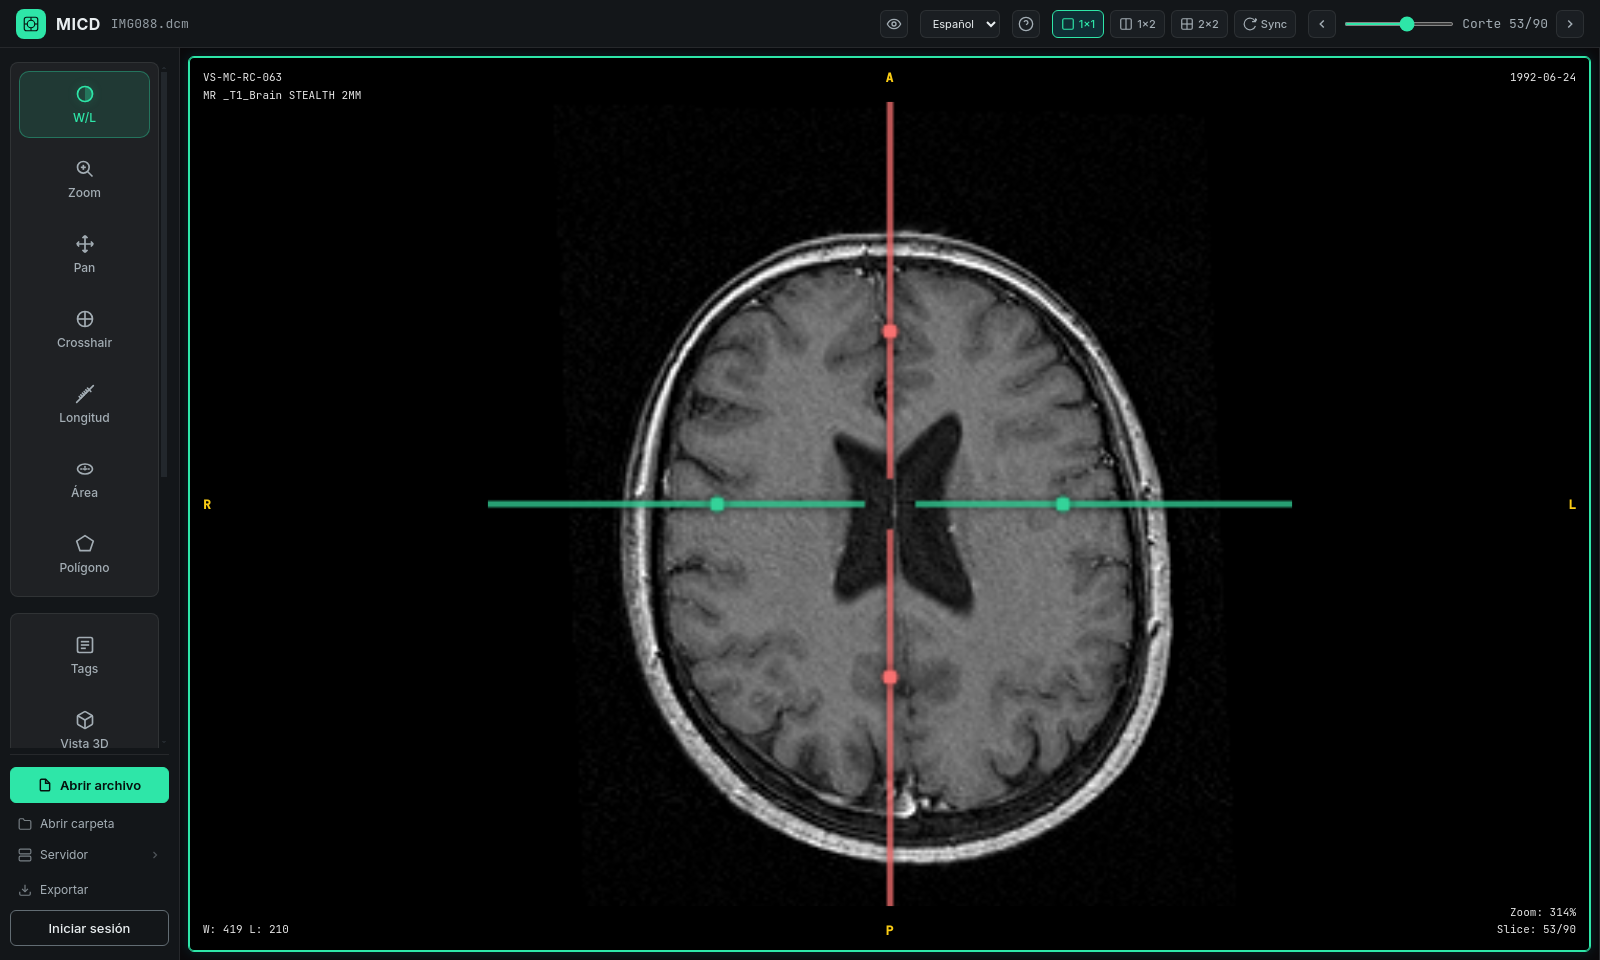
\includegraphics[width=\linewidth]{02-visor-serie}
  \end{tcolorbox}
  \end{center}

  \vfill
  \begin{minipage}[b]{0.6\linewidth}
    {\large\bfseries UBA — FIUBA\par}
    \vspace{3pt}
    {\color{white!70!micddark} Versión web (staging) — octubre de 2026\par}
  \end{minipage}
  \vspace*{0.3cm}
\end{titlepage}

\tableofcontents

% ════════════════════════════════════════════════════════════════════════════
\chapter{Bienvenida}

\section{¿Qué es MICD?}

MICD es un visor de imágenes médicas que funciona directamente en el navegador
de internet (Chrome, Firefox, Edge o Safari), sin instalar nada. Permite:

\begin{itemize}
  \item \textbf{Ver estudios} de tomografía, resonancia, radiografía y otras
        modalidades guardados en su computadora (formato DICOM).
  \item \textbf{Ajustar la imagen}: brillo y contraste (ventana), zoom,
        desplazamiento y navegación por los cortes de la serie.
  \item \textbf{Medir}: distancias, áreas con densidad media (UH) y regiones a
        mano alzada.
  \item \textbf{Reconstruir} la serie en los planos axial, coronal y sagital, y
        verla en 3D.
  \item \textbf{Trabajar con el servidor} del servicio: buscar estudios
        compartidos, subir estudios nuevos y validarlos con ayuda de una
        segmentación automática.
\end{itemize}

\section{Dos formas de uso}

\begin{description}[leftmargin=1em,style=nextline]
  \item[Sin iniciar sesión — visor local]
    Puede abrir imágenes de su propia computadora en cualquier momento. Las
    imágenes \textbf{no salen de su equipo}: se muestran en el navegador y nada
    se envía al servidor.
  \item[Con sesión iniciada — servidor]
    Con su usuario y contraseña accede a los estudios guardados en el servidor
    del servicio, puede subir estudios nuevos y validar estudios.
\end{description}

\section{Su perfil: Médico}

Cada persona tiene un perfil que define qué puede hacer. Esta guía está
escrita para el perfil \textbf{Médico}, que permite:

\begin{itemize}
  \item ver los estudios del servidor con los datos completos del paciente;
  \item subir estudios nuevos al servidor;
  \item aprobar, rechazar o marcar para revisión los estudios (validación);
  \item exportar imágenes y estudios.
\end{itemize}

Existen otros tres perfiles, descritos en el apéndice~\ref{ap:perfiles}:

\begin{center}
\rowcolors{2}{gray!8}{white}
\begin{tabularx}{\linewidth}{lX}
  \toprule
  \textbf{Perfil} & \textbf{Qué puede hacer} \\
  \midrule
  Médico & Ver, subir, validar y exportar estudios, con datos completos del paciente. \\
  Administrador & Todo lo anterior, más gestionar usuarios, ver la auditoría, configurar el servidor y publicar en Zenodo. \\
  Investigador & Ver estudios con los datos del paciente ocultos (anonimizados). No sube ni valida. \\
  Informático de clínica & Sólo subir y descargar estudios. No usa el visor. \\
  \bottomrule
\end{tabularx}
\end{center}

\section{Recorrido guiado dentro de la aplicación}

La primera vez que inicia sesión, MICD le ofrece un recorrido paso a paso que
resalta cada parte de la pantalla. Puede saltearlo con \btn{Omitir tutorial} o
con la tecla \tecla{Esc}, y volver a verlo cuando quiera con el botón
\btn{?} de la barra superior.

\captura[0.8]{14-tour-1}{Primer paso del recorrido guiado.}

% ════════════════════════════════════════════════════════════════════════════
\chapter{Primeros pasos}

\section{Abrir la aplicación}

Abra el navegador e ingrese la dirección que le indicó el área de sistemas de
su institución. Verá la pantalla principal del visor:

\captura{01-inicio}{Pantalla de inicio del visor, sin ninguna imagen abierta.}

La pantalla tiene tres zonas:

\begin{enumerate}
  \item \textbf{Barra superior}: nombre del estudio abierto, idioma, ayuda
        (\btn{?}), distribución de pantalla (\btn{1×1}, \btn{1×2}, \btn{2×2})
        y, cuando hay una serie abierta, el control para pasar de corte.
  \item \textbf{Barra lateral izquierda}: las herramientas (W/L, Zoom, Pan,
        mediciones, etc.) y, abajo, los botones \btn{Abrir archivo},
        \btn{Abrir carpeta}, \btn{Servidor}, \btn{Exportar} e
        \btn{Iniciar sesión}.
  \item \textbf{Zona central}: donde se muestra la imagen.
\end{enumerate}

\section{Cambiar el idioma}

La aplicación está disponible en \textbf{español} e \textbf{inglés}. Use el
selector de idioma de la barra superior (dice \btn{Español}). El cambio es
inmediato y se recuerda para la próxima vez.

\section{Iniciar sesión}

Para usar el servidor necesita iniciar sesión. Toque \btn{Iniciar sesión} (abajo
a la izquierda) o \btn{Servidor}. Aparece esta tarjeta:

\captura[0.85]{20-login}{Tarjeta de inicio de sesión.}

\begin{enumerate}
  \item Escriba su \textbf{email} y su \textbf{contraseña}. El ícono del ojo
        muestra u oculta la contraseña mientras la escribe.
  \item Toque \btn{Ingresar}.
\end{enumerate}

\begin{importante}
  Si se equivoca varias veces seguidas, por seguridad el sistema bloquea los
  intentos durante algunos minutos. Espere y vuelva a intentar.
\end{importante}

\section{Activar su cuenta por primera vez}

Cuando un administrador le crea la cuenta, usted recibe un email con un
\textbf{código de invitación} (vence a las 48 horas). Para activarla:

\begin{enumerate}
  \item Abra el enlace del email, \emph{o bien} en la tarjeta de inicio de
        sesión toque \btn{¿Te invitaron? Activá tu cuenta}.
  \item Escriba su email, el código recibido y elija una contraseña de al menos
        8 caracteres.
  \item Toque \btn{Crear cuenta e ingresar}. Quedará con la sesión iniciada.
\end{enumerate}

\captura[0.85]{22-activar-cuenta}{Activación de la cuenta con el código de invitación.}

\section{Si olvidó su contraseña}

\begin{enumerate}
  \item En la tarjeta de inicio de sesión toque \btn{¿Olvidaste tu contraseña?}.
  \item Escriba su email y toque \btn{Enviar código}. Recibirá un email con un
        código que vence en 1 hora.
  \item Abra el enlace del email, o vuelva a esta ventana y toque
        \btn{Ya tengo un código}.
  \item Escriba el código y su nueva contraseña. Al confirmar, ingresa
        directamente.
\end{enumerate}

\captura[0.85]{21-olvide-contrasena}{Recuperación de contraseña.}

\section{Su sesión}

Con la sesión iniciada, abajo a la izquierda verá sus iniciales, su email y el
tiempo restante de la sesión. El botón con la flecha cierra la sesión.

\begin{figure}[H]
  \centering
  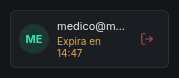
\includegraphics[width=0.35\linewidth]{28-sesion}
  \caption{Bloque de sesión: usuario, tiempo restante y botón para salir.}
\end{figure}

Si la sesión vence mientras trabaja, la próxima acción en el servidor le
pedirá iniciar sesión otra vez. Las imágenes que ya tiene abiertas no se
pierden.

\begin{importante}
  En computadoras compartidas (consultorio, guardia, sala de informes),
  \textbf{cierre siempre la sesión} al terminar.
\end{importante}

% ════════════════════════════════════════════════════════════════════════════
\chapter{Ver imágenes de su computadora}

\section{Abrir un estudio}

Tiene tres formas de abrir imágenes DICOM guardadas en su computadora:

\begin{itemize}
  \item \textbf{Arrastrar y soltar} los archivos \texttt{.dcm} (o la carpeta
        completa) sobre la zona central.
  \item Tocar \btn{Abrir archivo} o \btn{Seleccionar archivos} y elegir uno o
        varios archivos. Para abrir una serie completa, seleccione todos los
        archivos de la carpeta (\tecla{Ctrl}+\tecla{A}).
  \item Tocar \btn{Abrir carpeta} para abrir
        todos los archivos de una carpeta de una sola vez.
\end{itemize}

MICD ordena los cortes automáticamente y muestra el primero:

\captura{02-visor-serie}{Serie de resonancia abierta en el visor.}

Sobre la imagen se muestra información de referencia:

\begin{itemize}
  \item arriba a la izquierda, el paciente y la descripción de la serie;
  \item arriba a la derecha, la fecha del estudio;
  \item en los bordes, las letras de orientación (\textbf{A} anterior,
        \textbf{P} posterior, \textbf{R} derecha del paciente, \textbf{L}
        izquierda);
  \item abajo a la izquierda, la ventana actual (\textbf{W} ancho y \textbf{L}
        nivel);
  \item abajo a la derecha, el zoom y el número de corte.
\end{itemize}

Las líneas de color que cruzan la imagen indican la posición de los otros
planos (coronal y sagital) y se usan en la reconstrucción multiplanar
(capítulo~\ref{cap:mpr}).

\section{Pasar de un corte a otro}

\begin{itemize}
  \item Arrastre el control deslizante de la barra superior
        (\btn{Corte 53/90}), o use las flechas \btn{<} y \btn{>} a sus lados.
  \item Con el teclado: \tecla{Re Pág} y \tecla{Av Pág}.
\end{itemize}

\section{Brillo y contraste (ventana W/L)}

La herramienta \btn{W/L} está activa al abrir un estudio. Para ajustar la
imagen:

\begin{itemize}
  \item \textbf{Arrastre con el mouse sobre la imagen}: horizontal cambia el
        contraste (ancho de ventana) y vertical cambia el brillo (nivel).
  \item O toque otra vez \btn{W/L} para abrir el panel con los controles
        deslizantes y los \textbf{presets}: \btn{Pulmón}, \btn{Hueso},
        \btn{Tejido Blando} y \btn{Cerebro}.
\end{itemize}

\captura{03-panel-wl}{Panel de ajuste de ventana con los presets.}

\begin{consejo}
  Los presets usan valores de tomografía (unidades Hounsfield). En resonancia
  conviene ajustar la ventana arrastrando sobre la imagen.
\end{consejo}

\section{Zoom y desplazamiento}

\begin{itemize}
  \item \btn{Zoom}: arrastre hacia arriba o abajo sobre la imagen para acercar o
        alejar. También puede usar la rueda del mouse. Al tocar \btn{Zoom}
        otra vez se abre un panel con los accesos \btn{Ajustar a pantalla},
        \btn{100\%} y \btn{200\%}.
  \item \btn{Pan}: arrastre la imagen para moverla dentro de la pantalla.
  \item \btn{Reset}: vuelve la ventana, el zoom y la posición a los valores
        iniciales.
\end{itemize}

\captura{05-zoom}{Panel de zoom con los accesos rápidos.}

\section{Ocultar la información superpuesta}

El botón con forma de \textbf{ojo} en la barra superior oculta o muestra los
textos sobre la imagen (paciente, fecha, ventana, etc.). Es útil para ver la
imagen limpia o para mostrarla en una presentación.

\captura{06-sin-info}{Imagen sin los textos superpuestos.}

\section{Ver varias imágenes a la vez}

Los botones \btn{1×1}, \btn{1×2} y \btn{2×2} de la barra superior dividen la
zona central en uno, dos o cuatro cuadros. Toque un cuadro para activarlo:
las herramientas actúan sobre el cuadro activo (marcado con borde verde). El
botón \btn{Sync} sincroniza el desplazamiento entre cuadros.

\captura{10-layout-2x2}{Distribución en cuatro cuadros (2×2).}

\section{Ver las etiquetas DICOM}

El botón \btn{Tags} (o la tecla \tecla{M}) abre a la derecha un panel con los
datos del estudio: paciente, fecha, descripción, modalidad, serie,
dimensiones de la imagen, tamaño del píxel, etc.

\captura{09-etiquetas}{Panel de etiquetas DICOM.}

\section{Atajos de teclado}

\begin{center}
\rowcolors{2}{gray!8}{white}
\begin{tabular}{ll}
  \toprule
  \textbf{Tecla} & \textbf{Acción} \\
  \midrule
  \tecla{W} & Herramienta brillo/contraste (W/L) \\
  \tecla{Z} & Herramienta zoom \\
  \tecla{P} & Herramienta desplazamiento (Pan) \\
  \tecla{C} & Navegación con cruz (en vistas 3D/MPR) \\
  \tecla{L} & Medir longitud \\
  \tecla{E} & Medir área \\
  \tecla{$\leftarrow$}\,\tecla{$\uparrow$}\,\tecla{$\downarrow$}\,\tecla{$\rightarrow$} & Ajustan la herramienta activa (con \tecla{Shift}, pasos grandes) \\
  \tecla{Re Pág} / \tecla{Av Pág} & Corte anterior / siguiente \\
  \tecla{R} & Restablecer la vista \\
  \tecla{M} & Mostrar u ocultar las etiquetas DICOM \\
  \tecla{Esc} & Cerrar ventanas y el recorrido guiado \\
  \bottomrule
\end{tabular}
\end{center}

% ════════════════════════════════════════════════════════════════════════════
\chapter{Mediciones y marcado de regiones}

Las herramientas de medición están en la barra lateral: \btn{Longitud},
\btn{Área} y \btn{Polígono}. Al elegir cualquiera se abre el panel
\textbf{Ajuste de Mediciones}, donde puede:

\begin{itemize}
  \item elegir las unidades (\btn{mm} o \btn{cm});
  \item asignar una \textbf{patología} a una región marcada;
  \item cambiar el grosor de la línea;
  \item \btn{Esconder/Mostrar} las mediciones;
  \item \btn{Guardar} las mediciones;
  \item \btn{Exportar Segmentación} de las regiones marcadas;
  \item \btn{Borrar mediciones} del corte.
\end{itemize}

\section{Medir una distancia}

\begin{enumerate}
  \item Toque \btn{Longitud} (o la tecla \tecla{L}).
  \item Haga clic en el punto inicial, mantenga apretado y suelte en el punto
        final.
  \item La distancia aparece sobre la línea, en milímetros.
\end{enumerate}

\captura{07-medicion-longitud}{Medición de una distancia (104,3 mm).}

\section{Medir un área y su densidad}

\begin{enumerate}
  \item Toque \btn{Área} (o la tecla \tecla{E}).
  \item Arrastre para dibujar una elipse sobre la región de interés.
  \item Se muestra el \textbf{área} en mm² y la \textbf{media} de la región con
        su desvío estándar (en tomografía, en unidades Hounsfield).
\end{enumerate}

\captura{08-medicion-area}{Medición de área con valor medio.}

\section{Marcar una región a mano (polígono)}

\begin{enumerate}
  \item Toque \btn{Polígono}.
  \item Haga clic punto por punto siguiendo el contorno de la región.
  \item Para cerrar la figura, haga clic otra vez sobre el primer punto.
  \item Con el polígono seleccionado, puede asignarle una patología desde el
        panel de mediciones.
\end{enumerate}

\captura{36-poligono}{Región marcada con la herramienta Polígono, con su área y perímetro.}

\begin{importante}
  Si el estudio no tiene la información de calibración espacial, la medición
  muestra el aviso \emph{``Sin calibración espacial''} y los valores no
  deben usarse como medidas reales.
\end{importante}

% ════════════════════════════════════════════════════════════════════════════
\chapter{Reconstrucción multiplanar y vista 3D}
\label{cap:mpr}

Estas herramientas necesitan una serie de varios cortes (por ejemplo, una
tomografía o resonancia volumétrica).

\section{Reconstrucción multiplanar (MPR)}

Toque \btn{MPR} en la barra lateral. La pantalla se divide en una grilla de
cuatro cuadros:

\begin{itemize}
  \item arriba a la izquierda, el corte \textbf{axial} (el original);
  \item arriba a la derecha, la reconstrucción \textbf{coronal};
  \item abajo a la izquierda, la reconstrucción \textbf{sagital};
  \item abajo a la derecha, el \textbf{volumen 3D} con los tres planos
        dibujados, para ubicarse en el espacio.
\end{itemize}

\captura{12-mpr}{Reconstrucción multiplanar: axial, coronal, sagital y volumen 3D.}

Las líneas de color sobre cada cuadro marcan dónde cortan los otros planos.
Con la herramienta \btn{Crosshair} (tecla \tecla{C}) haga clic en un punto de
cualquier cuadro, o arrastre los puntos de las líneas: los demás planos se
mueven para mostrar ese mismo punto. Los controles deslizantes de la esquina
superior derecha (\textbf{Axial}, \textbf{Coronal}, \textbf{Sagital}) recorren
cada plano corte por corte.

\section{Vista 3D}

Toque \btn{Vista 3D}. Se muestra el volumen completo con los tres planos de
corte. Abajo a la derecha puede elegir \btn{Axial}, \btn{Sagital},
\btn{Coronal} o \btn{Vista Volumétrica}; los controles deslizantes de la
esquina superior derecha mueven cada plano. El cubo de abajo a la izquierda
indica la orientación.

\captura{13-vista-3d}{Vista volumétrica 3D.}

Para volver a la vista normal, toque otra vez el mismo botón (\btn{MPR} o
\btn{Vista 3D}).

\begin{consejo}
  Si aparece un aviso de que el estudio no es compatible, la serie tiene un
  solo corte o le faltan datos de posición. Si el aviso menciona
  \emph{WebGL2}, pruebe con una versión actualizada de Chrome o Edge.
\end{consejo}

% ════════════════════════════════════════════════════════════════════════════
\chapter{Exportar imágenes y estudios}

Toque \btn{Exportar} en la barra lateral. Puede elegir:

\begin{itemize}
  \item \btn{Exportar vista actual (PNG)}: guarda una imagen tal como se ve
        en pantalla, con el ajuste de ventana y las mediciones. Ideal para
        presentaciones o ateneos.
  \item \btn{Exportar estudio completo (ZIP)}: guarda todos los archivos
        DICOM del estudio en un archivo comprimido.
\end{itemize}

\captura{11-exportar}{Opciones de exportación.}

\begin{importante}
  El estudio exportado en ZIP se \textbf{anonimiza} automáticamente: se quitan
  el nombre, el documento y otros datos que identifican al paciente. Aun así,
  revise la imagen PNG antes de compartirla: si el paciente aparece en los
  textos de la pantalla, oculte la información con el botón del ojo antes de
  exportar.
\end{importante}

% ════════════════════════════════════════════════════════════════════════════
\chapter{Estudios del servidor}

El botón \btn{Servidor} abre la pantalla del servidor, que tiene tres pestañas:
\btn{Buscar}, \btn{Cargar} y \btn{Validaciones}. Para volver al visor use
\btn{< Volver al visualizador}, arriba a la izquierda.

\section{Buscar un estudio}

\captura{23-buscar}{Pestaña Buscar con los estudios del servidor.}

Para encontrar un estudio puede combinar:

\begin{itemize}
  \item el buscador \btn{Buscar paciente o ID} (nombre o identificación del
        paciente);
  \item un rango de fechas (\textbf{Desde} / \textbf{Hasta});
  \item el campo \btn{Filtrar por descripción};
  \item los botones de \textbf{modalidad}: \btn{CT}, \btn{MR}, \btn{RX},
        \btn{CR}, \btn{US}, \btn{NM}, \btn{PET}, \btn{MG}, \btn{XA}, o
        \btn{Todas}.
\end{itemize}

Cada tarjeta muestra el paciente, la fecha, la descripción, la modalidad, la
cantidad de imágenes y su clasificación. Los estudios subidos recientemente
llevan la marca \btn{Nuevo}.

\section{Abrir un estudio del servidor}

\begin{enumerate}
  \item Toque la tarjeta del estudio para seleccionarla (queda resaltada).
  \item Toque \btn{Abrir estudio seleccionado}, abajo a la derecha.
\end{enumerate}

\captura{24-estudio-seleccionado}{Estudio seleccionado, listo para abrir.}

El estudio se descarga y se abre en el visor. Todas las herramientas de los
capítulos anteriores funcionan igual.

\captura{25-visor-servidor}{Estudio del servidor abierto en el visor.}

\section{Panel lateral de estudios}

Mientras mira un estudio, puede abrir la lista de estudios del servidor sin
salir del visor: toque \btn{Estudios} en la barra lateral. A la derecha
aparece un panel con los mismos filtros; un clic en un estudio lo abre de
inmediato. También puede arrastrar archivos sobre este panel para subirlos.

\captura{27-panel-estudios}{Panel lateral «Estudios en servidor».}

% ════════════════════════════════════════════════════════════════════════════
\chapter{Subir estudios al servidor}

\section{Los estudios se anonimizan antes de salir de su computadora}

Por protección de los datos de los pacientes, \textbf{ningún estudio sale de
su computadora con datos identificatorios}. Antes de enviar cada archivo,
MICD lo pasa por un \textbf{programa de anonimización} instalado en su propia
computadora, que quita el nombre, el documento y los demás datos personales.
Al servidor sólo llega la copia anonimizada.

\begin{importante}
  Para subir estudios, el programa de anonimización tiene que estar instalado
  y funcionando en su computadora. Si no lo está, MICD \textbf{no envía nada}
  y muestra el mensaje \emph{``No se puede subir: no se pudo anonimizar el
  estudio. Contactá a un administrador.''} En ese caso pida al área de
  sistemas que lo instale o lo inicie.
\end{importante}

\captura{37-anonimizador-no-disponible}{Aviso cuando el programa de anonimización no está disponible: no se sube nada.}

Además, el servidor vuelve a revisar cada imagen recibida. Si todavía
encuentra datos identificatorios, la rechaza (\emph{``El estudio conserva
datos identificatorios y no se guardó''}) o la guarda marcada para revisión,
según cómo lo haya configurado la institución.

\section{Cómo subir un estudio}

\begin{enumerate}
  \item Vaya a \btn{Servidor} y abra la pestaña \btn{Cargar}.
  \item Arrastre a la zona punteada los archivos \texttt{.dcm}, un archivo
        \texttt{.zip} o una carpeta completa; o toque
        \btn{Seleccionar archivos o ZIP}.
  \item Se abre la ventana \textbf{Clasificar estudio}. Elija una
        clasificación (opcional): \textit{ACV, Hemorragia, Tumor,
        Desmielinizante, Normales, Otros} o \textit{Sin clasificar}.
  \item Toque \btn{Subir}. Si toca \btn{Cancelar}, no se envía nada.
  \item Un panel muestra el avance de toda la carga: el porcentaje total, el
        paso actual (\emph{``Anonimizando archivo 1 de 3''}, luego
        \emph{``Subiendo archivo 1 de 3''}), los megabytes enviados y el
        tiempo restante estimado.
  \item Al terminar verá \emph{``Carga completa''} (o \emph{``Carga terminada
        con errores''}, con el enlace \btn{Ver archivos con problemas}).
        Toque \btn{Finalizar}.
\end{enumerate}

\captura{29-cargar}{Pestaña Cargar.}

\captura{30-clasificar}{Clasificación del estudio antes de subirlo.}

\captura{38-progreso-carga}{Panel de avance de la carga: porcentaje, paso actual y tamaño.}

\section{Qué tener en cuenta}

\begin{itemize}
  \item Cada archivo puede pesar hasta \textbf{2 GB}.
  \item Si un estudio \textbf{ya existe} en el servidor, MICD le pregunta qué
        hacer: \btn{Reemplazar}, \btn{Cancelar} (omitir ese estudio) o
        \btn{Cancelar todo}. Su elección se aplica a todos los archivos
        repetidos de esa carga.
  \item Debajo de la zona de carga se indica si la conexión es
        \textbf{cifrada (HTTPS)}. Si dice \emph{``Conexión sin cifrar (HTTP) —
        sólo para uso local''}, no suba estudios con datos reales de
        pacientes desde fuera de la red de la institución y avise al área de
        sistemas.
  \item Puede detener una carga en curso con \btn{Cancelar}: los archivos que
        todavía no se enviaron no se suben.
  \item También puede subir arrastrando archivos sobre el panel lateral
        \textbf{Estudios en servidor} del visor.
\end{itemize}

% ════════════════════════════════════════════════════════════════════════════
\chapter{Validar estudios}

La validación es el registro de su opinión profesional sobre un estudio:
\textbf{aprobado}, \textbf{rechazado} o \textbf{marcado para revisión}. Queda
registrado quién validó y cuándo.

\section{La lista de validaciones}

Abra \btn{Servidor} y la pestaña \btn{Validaciones}. La tabla muestra cada
estudio con su paciente, modalidad, fecha, estado y quién lo validó. Los
botones de arriba filtran por estado: \btn{Todos}, \btn{Sin validar},
\btn{Aprobados}, \btn{Rechazados} y \btn{Para revisión}.

\captura{31-validaciones}{Pestaña Validaciones.}

\section{Revisar un estudio con la segmentación automática}

Toque \btn{Segmentar con IA} en la fila del estudio. El estudio se abre en el
visor en dos cuadros:

\begin{itemize}
  \item a la izquierda, la \textbf{imagen original};
  \item a la derecha, la misma imagen con la \textbf{región propuesta por la
        IA}, con su área y perímetro.
\end{itemize}

Abajo aparece la \textbf{barra de validación}:

\captura{33-segmentacion-ia}{Estudio abierto para validar, con la segmentación propuesta por la IA.}

\begin{importante}
  La segmentación automática es una \textbf{ayuda} para la lectura y en esta
  versión es \textbf{simulada} (de demostración). No reemplaza su criterio
  clínico: revise siempre la imagen original.
\end{importante}

\section{Corregir la segmentación}

Si el contorno propuesto no es correcto:

\begin{enumerate}
  \item Toque \btn{Corregir}. Aparecen los puntos (vértices) del contorno.
  \item Arrastre los puntos para ajustar el contorno; también puede agregar o
        quitar puntos.
  \item Toque \btn{Enviar} para guardar la corrección, o \btn{Cancelar} para
        dejarla como estaba.
\end{enumerate}

\captura{34-corregir-segmentacion}{Modo de corrección: los puntos del contorno se pueden mover.}

Otros botones de la barra:

\begin{itemize}
  \item \btn{Descartar corrección}: vuelve al contorno original de la IA.
  \item \btn{$\rightarrow$ Transferir al original}: copia la segmentación sobre la imagen
        original para verla en la vista común (se puede revertir).
  \item \btn{Descartar}: descarta la segmentación de la IA sin tocar la
        imagen original (se puede restaurar).
  \item El selector de \textbf{clasificación} (\btn{Sin clasificar}) permite
        indicar el tipo de patología.
\end{itemize}

\section{Aprobar, rechazar o marcar para revisión}

\begin{enumerate}
  \item Toque \btn{Aprobar}, \btn{Rechazar} o \btn{Marcar para revisión}.
  \item Se abre una ventana de confirmación. Al rechazar, se recomienda dejar
        un \textbf{comentario} explicando el motivo.
  \item Toque \btn{Confirmar}.
\end{enumerate}

\captura{26-validar-dialogo}{Confirmación de un rechazo, con su comentario.}

\begin{consejo}
  Una vez validado un estudio, sólo un administrador puede registrar una
  corrección de esa validación. Si se equivocó, avise a un administrador.
\end{consejo}

% ════════════════════════════════════════════════════════════════════════════
\chapter{Otras funciones}

\section{Capas}

El botón \btn{Capas} permite superponer otro estudio sobre el actual
(\btn{Cargar Estudio Superpuesto}) y ajustar su opacidad y su ventana. Es útil
para comparar dos adquisiciones del mismo paciente.

\section{Zenodo: conjuntos de imágenes públicos}

Zenodo es un repositorio público donde se publican conjuntos de imágenes para
investigación. El botón \btn{Zenodo} (al final de la barra lateral; tenga un
estudio abierto para verlo) abre un panel a la derecha.

\captura{47-zenodo-buscar}{Búsqueda de conjuntos de imágenes en Zenodo.}

\subsection*{Buscar e importar}

\begin{enumerate}
  \item En la pestaña \btn{Buscar}, escriba términos como
        \emph{``CT lung''} o \emph{``brain MRI''} y toque \btn{Buscar}. Puede
        filtrar por tipo de archivo (\btn{Todos}, \btn{DCM}, \btn{ZIP}).
  \item Cada resultado muestra título, autores, año, tamaño y cantidad de
        archivos. Los que dicen \emph{``No importable''} no contienen
        imágenes DICOM.
  \item Toque \btn{Importar} (o \btn{Importar ZIP}) para traer el conjunto al
        servidor. Los archivos grandes pueden tardar varios minutos.
  \item Si ya conoce el identificador del conjunto (DOI, por ejemplo
        \texttt{10.5281/zenodo.1234567}), péguelo arriba y toque
        \btn{Importar por DOI}.
\end{enumerate}

Los estudios importados aparecen en la búsqueda del servidor con la marca
\btn{Importado}. Al seleccionarlos en \btn{Buscar} se ve su información de
Zenodo (autores, fecha, descargas, historial de versiones) y se puede
\btn{Verificar actualización en Zenodo} o \btn{Importar versión más reciente}.

\begin{consejo}
  Publicar en Zenodo y configurar la conexión son tareas del administrador
  (ver el apéndice~\ref{ap:admin}).
\end{consejo}

% ════════════════════════════════════════════════════════════════════════════
\chapter{Preguntas frecuentes}

\begin{description}[leftmargin=0pt,style=nextline,itemsep=8pt]
  \item[¿Necesito iniciar sesión para ver una imagen de mi computadora?]
    No. Ver archivos locales funciona sin sesión y las imágenes no se envían
    a ningún lado.

  \item[Abrí un archivo y aparece «No se encontraron datos de píxeles».]
    El archivo usa un formato comprimido que el navegador no puede leer.
    Pruebe con la versión de escritorio o pida el estudio sin compresión.

  \item[Elegí una carpeta y dice que no hay archivos DICOM.]
    La carpeta no contiene archivos DICOM válidos. Verifique que sea la
    carpeta de las imágenes y no, por ejemplo, la de un visor que viene en el
    CD del paciente.

  \item[La reconstrucción MPR o la vista 3D no se activan.]
    Necesitan una serie con más de un corte e información de posición. Las
    radiografías simples no se pueden reconstruir.

  \item[Me pidió iniciar sesión otra vez en medio del trabajo.]
    La sesión venció. Vuelva a ingresar: el estudio abierto se conserva.

  \item[No veo la pestaña Usuarios ni Sistema.]
    Son exclusivas del perfil Administrador.

  \item[«Demasiados intentos».]
    Por seguridad, después de varios intentos fallidos hay que esperar
    algunos minutos.

  \item[¿Quién ve los datos del paciente?]
    Los perfiles Médico, Administrador e Informático de clínica. El perfil
    Investigador ve los estudios anonimizados, y toda exportación en ZIP se
    anonimiza.

  \item[No puedo subir: «no se pudo anonimizar el estudio».]
    El programa de anonimización de su computadora no está instalado o no
    está funcionando. No se envió nada. Pida ayuda al área de sistemas.

  \item[Subí un estudio y dice «conserva datos identificatorios».]
    El servidor encontró datos personales que la anonimización no quitó y no
    lo guardó. Avise al administrador indicando qué estudio era.

  \item[No veo el panel de Zenodo al tocar el botón.]
    Abra primero un estudio: con el visor vacío, el panel queda tapado.
\end{description}

\section*{Soporte}

Ante cualquier problema, comuníquese con el administrador de MICD de su
institución indicando qué estaba haciendo, el mensaje que apareció y, si es
posible, una captura de pantalla \textbf{sin datos del paciente}.

% ════════════════════════════════════════════════════════════════════════════
\appendix

\chapter{Otros perfiles}
\label{ap:perfiles}

\section{Administrador}
\label{ap:admin}

El administrador tiene todas las funciones del médico y, además, en la
pantalla \btn{Servidor} ve las pestañas \btn{Usuarios} y \btn{Sistema} y el
botón de engranaje (arriba a la derecha).

\subsection*{Gestionar usuarios}

\captura{40-usuarios}{Pestaña Usuarios: cuentas, perfiles, estado y último acceso.}

\begin{itemize}
  \item \textbf{Crear un usuario}: complete \textbf{Nombre}, \textbf{Correo} y
        \textbf{Rol}, y toque \btn{Crear usuario}. La persona recibe por email
        un código de invitación para activar su cuenta (vence a las 48 horas).
  \item \textbf{Cambiar el perfil}: elija otro rol en la lista de la fila del
        usuario. El cambio se aplica por completo en hasta 15 minutos.
  \item \btn{Bloquear} / \btn{Habilitar}: suspende el acceso de una cuenta y
        cierra sus sesiones; se puede volver a habilitar.
  \item \btn{Eliminar}: quita la cuenta, pero conserva su historial de
        auditoría. La cuenta puede volver a crearse más adelante.
  \item La columna \textbf{Último acceso} muestra cuándo ingresó cada persona.
  \item \btn{Descargar log de auditoría (CSV)}: descarga el registro de
        acciones sobre usuarios para revisarlo en una planilla.
\end{itemize}

\captura{41-crear-usuario}{Alta de un usuario nuevo.}

\subsection*{Historial de actividad}

En el panel lateral \textbf{Estudios en servidor} del visor, el administrador
tiene un botón de historial que abre el registro de actividad: quién vio,
descargó o subió cada estudio, y cuándo.

\captura{44-actividad}{Historial de actividad (auditoría de accesos a estudios).}

\subsection*{Sistema y configuración del servidor}

\begin{itemize}
  \item La pestaña \btn{Sistema} muestra el espacio ocupado y libre del
        almacenamiento de imágenes y la cantidad de estudios, series e
        imágenes guardadas. Cuando el espacio está por agotarse, la aplicación
        muestra un aviso.
  \item El botón de \textbf{engranaje} abre \textbf{Configuración del
        Servidor}, donde se indica la dirección del servidor. Cámbiela sólo
        con indicación del área de sistemas.
\end{itemize}

\captura{42-sistema}{Pestaña Sistema: uso del almacenamiento.}

\captura{43-config-servidor}{Configuración de la dirección del servidor.}

\subsection*{Zenodo: configuración y publicación}

\begin{itemize}
  \item Pestaña \btn{Config} del panel Zenodo: cargar el \textbf{token} de
        acceso para los entornos de prueba (\textit{Sandbox}) y
        \textit{Producción}, y programar la \textbf{sincronización}
        (6 h, 12 h, 24 h, semanal o desactivada) que busca versiones nuevas de
        los estudios importados. \btn{Sincronizar ahora} la ejecuta en el
        momento.
  \item Pestaña \btn{Publicar}: con un estudio seleccionado en el panel de
        estudios, complete título, descripción, autores y palabras clave, y
        toque \btn{Publicar en Zenodo}. El estudio tiene que estar
        anonimizado.
  \item Pestaña \btn{Logs}: historial de publicaciones e importaciones, que
        se puede filtrar y descargar en CSV.
\end{itemize}

\captura{48-zenodo-config}{Configuración de Zenodo: tokens y sincronización.}

\begin{importante}
  Publicar en Zenodo es \textbf{irreversible} y deja los datos disponibles
  públicamente en internet. Revise con cuidado antes de publicar.
\end{importante}

\subsection*{Corregir una validación}

Si un estudio ya fue validado, sólo el administrador puede registrar una
\textbf{corrección}. Al abrir el estudio desde \btn{Validaciones}, la barra
avisa \emph{``Esto registrará una corrección sobre la validación previa''} y
los botones \btn{Aprobar}, \btn{Rechazar} y \btn{Marcar para revisión} dejan
registrada la corrección sin borrar la validación original.

\section{Investigador}

El investigador puede buscar y ver estudios, pero \textbf{nunca ve datos
identificatorios}: el nombre aparece como \textit{ANONYMIZED}, la
identificación del paciente se reemplaza por un código y la búsqueda por
nombre está desactivada. Las imágenes que descarga también llegan
anonimizadas. No puede subir estudios, validarlos ni publicar en Zenodo,
pero sí buscar en el repositorio público de Zenodo.

\captura{45-investigador-buscar}{Lo que ve un investigador: estudios con datos del paciente ocultos.}

\begin{importante}
  La anonimización quita los datos de las etiquetas DICOM, pero \textbf{no}
  el texto que esté ``quemado'' dentro de la imagen (habitual en ecografías y
  capturas de pantalla). Téngalo en cuenta antes de compartir esas imágenes.
\end{importante}

\section{Informático de clínica}

Perfil para el personal de sistemas que mueve estudios entre equipos. Al
iniciar sesión entra directamente a la pantalla del servidor, sin visor, con
dos pestañas:

\begin{itemize}
  \item \btn{Buscar}: seleccione un estudio y toque
        \btn{Descargar estudio seleccionado} para bajarlo como \texttt{.zip}.
  \item \btn{Cargar}: suba estudios igual que en el capítulo de carga
        (también pasan por la anonimización).
\end{itemize}

Para salir, use \btn{Cerrar sesión} arriba a la derecha.

\captura{46-informatico}{Pantalla del informático de clínica, con el botón de descarga.}

% ════════════════════════════════════════════════════════════════════════════
\chapter{Casos de uso cubiertos}
\label{ap:cobertura}

Esta tabla enumera las funciones de MICD que usa una persona (versión
\texttt{staging} de la aplicación web y del servidor) e indica dónde se
explica cada una en esta guía.

\newcommand{\si}{\textcolor{micd}{\textbf{Sí}}}
\newcommand{\parcial}{\textcolor{orange!80!black}{\textbf{Parcial}}}

{\small
\rowcolors{2}{gray!8}{white}
\begin{longtable}{p{0.6cm}p{8.6cm}p{4.2cm}p{1.4cm}}
  \toprule
  \textbf{\#} & \textbf{Caso de uso} & \textbf{Dónde} & \textbf{Cubierto} \\
  \midrule
  \endhead
  \multicolumn{4}{l}{\textit{Acceso y cuenta}} \\
  1 & Iniciar sesión & Primeros pasos & \si \\
  2 & Activar la cuenta con el código de invitación & Primeros pasos & \si \\
  3 & Recuperar la contraseña & Primeros pasos & \si \\
  4 & Ver el tiempo de sesión y cerrar sesión & Primeros pasos & \si \\
  5 & Cambiar el idioma & Primeros pasos & \si \\
  6 & Recorrido guiado y volver a verlo & Bienvenida & \si \\
  \multicolumn{4}{l}{\textit{Visor}} \\
  7 & Abrir archivos locales o arrastrarlos & Ver imágenes & \si \\
  8 & Abrir una carpeta completa & Ver imágenes & \si \\
  9 & Pasar de corte & Ver imágenes & \si \\
  10 & Ajustar brillo/contraste y usar presets & Ver imágenes & \si \\
  11 & Zoom & Ver imágenes & \si \\
  12 & Desplazar la imagen (Pan) & Ver imágenes & \si \\
  13 & Restablecer la vista & Ver imágenes & \si \\
  14 & Ocultar la información superpuesta & Ver imágenes & \si \\
  15 & Varias imágenes a la vez (1×2, 2×2, Sync) & Ver imágenes & \si \\
  16 & Ver las etiquetas DICOM & Ver imágenes & \si \\
  17 & Atajos de teclado & Ver imágenes & \si \\
  18 & Medir una distancia & Mediciones & \si \\
  19 & Medir un área y su densidad media & Mediciones & \si \\
  20 & Marcar una región (polígono) y asignar patología & Mediciones & \si \\
  21 & Guardar, ocultar, borrar y exportar mediciones & Mediciones & \si \\
  22 & Reconstrucción multiplanar con navegación en cruz & MPR y 3D & \si \\
  23 & Vista volumétrica 3D & MPR y 3D & \si \\
  24 & Superponer otro estudio (capas) & Otras funciones & \parcial \\
  25 & Exportar la vista en PNG & Exportar & \si \\
  26 & Exportar el estudio en ZIP anonimizado & Exportar & \si \\
  \multicolumn{4}{l}{\textit{Servidor}} \\
  27 & Buscar y filtrar estudios & Estudios del servidor & \si \\
  28 & Abrir un estudio del servidor & Estudios del servidor & \si \\
  29 & Panel lateral de estudios & Estudios del servidor & \si \\
  30 & Requisito de anonimización antes de subir & Subir estudios & \si \\
  31 & Subir con clasificación y seguir el avance & Subir estudios & \si \\
  32 & Resolver estudios duplicados & Subir estudios & \si \\
  33 & Cancelar una carga & Subir estudios & \si \\
  34 & Rechazo del servidor por datos identificatorios & Subir estudios & \si \\
  35 & Lista de validaciones y filtros & Validar estudios & \si \\
  36 & Revisar con segmentación de IA & Validar estudios & \si \\
  37 & Corregir la segmentación & Validar estudios & \si \\
  38 & Transferir o descartar la segmentación & Validar estudios & \si \\
  39 & Aprobar, rechazar o marcar para revisión & Validar estudios & \si \\
  40 & Buscar en Zenodo e importar (también por DOI) & Otras funciones & \si \\
  41 & Ver datos de Zenodo de un estudio y buscar versiones nuevas & Otras funciones & \si \\
  \multicolumn{4}{l}{\textit{Administrador}} \\
  42 & Crear usuarios (invitación) & Apéndice A & \si \\
  43 & Cambiar el perfil de un usuario & Apéndice A & \si \\
  44 & Bloquear y habilitar cuentas & Apéndice A & \si \\
  45 & Eliminar cuentas & Apéndice A & \si \\
  46 & Descargar el log de auditoría (CSV) & Apéndice A & \si \\
  47 & Historial de actividad de estudios & Apéndice A & \si \\
  48 & Ver el almacenamiento del sistema & Apéndice A & \si \\
  49 & Configurar la dirección del servidor & Apéndice A & \si \\
  50 & Configurar Zenodo (tokens y sincronización) & Apéndice A & \si \\
  51 & Publicar un estudio en Zenodo & Apéndice A & \parcial \\
  52 & Historial de Zenodo (Logs) & Apéndice A & \parcial \\
  53 & Corregir una validación & Apéndice A & \si \\
  \multicolumn{4}{l}{\textit{Investigador e Informático de clínica}} \\
  54 & Buscar y ver estudios anonimizados & Apéndice A & \si \\
  55 & Pantalla de servidor del informático & Apéndice A & \si \\
  56 & Descargar un estudio seleccionado (ZIP) & Apéndice A & \si \\
  57 & Subir estudios como informático & Apéndice A & \si \\
  \bottomrule
\end{longtable}
}

\textbf{Resultado:} 54 de 57 casos de uso cubiertos por completo (95\%) y 3
de forma parcial, es decir, explicados en texto pero sin un paso a paso
completo con captura. Ningún caso de uso queda sin cubrir.

\end{document}
